\begin{figure}
\centering
\begin{subfigure}[b]{.3\textwidth}
\centering
\resizebox{\textwidth}{!}{
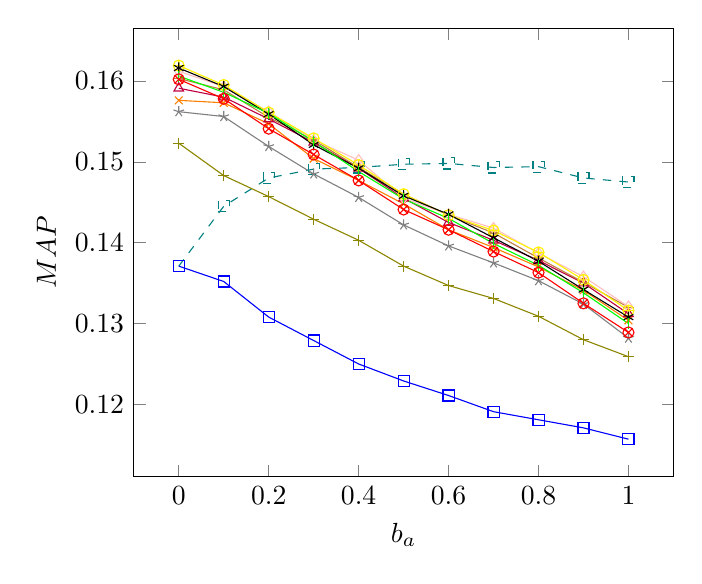
\begin{tikzpicture}
\begin{axis}[
xlabel=$b_a$,
ylabel=$MAP$,
% y label style={rotate=-90}
]

%%%%%%%%%%%
%% x = b_v, y = b_a
%%%%%%%%%%%
%\addplot[mark=square, style=solid, color=blue] coordinates
%{ (0.0,  0.1371 ) (0.1,  0.1523 ) (0.2,  0.1562 ) (0.3,  0.1576 ) (0.4,  0.1591 ) (0.5,  0.1603 ) (0.6,  0.1612 ) (0.7,  0.1619 ) (0.8,  0.1616 ) (0.9,  0.1606 ) (1.0,  0.1602 ) };

%\addplot[mark=+, style=solid, color=olive] coordinates
%{ (0.0,  0.1352 ) (0.1,  0.1483 ) (0.2,  0.1556 ) (0.3,  0.1573 ) (0.4,  0.158 ) (0.5,  0.1589 ) (0.6,  0.1593 ) (0.7,  0.1595 ) (0.8,  0.1593 ) (0.9,  0.1586 ) (1.0,  0.1578 ) };

%\addplot[mark=star, style=solid, color=gray] coordinates
%{ (0.0,  0.1308 ) (0.1,  0.1457 ) (0.2,  0.1519 ) (0.3,  0.1547 ) (0.4,  0.1553 ) (0.5,  0.1555 ) (0.6,  0.1562 ) (0.7,  0.1561 ) (0.8,  0.1559 ) (0.9,  0.156 ) (1.0,  0.1541 ) };

%\addplot[mark=x, style=solid, color=orange] coordinates
%{ (0.0,  0.1279 ) (0.1,  0.1429 ) (0.2,  0.1485 ) (0.3,  0.1504 ) (0.4,  0.1524 ) (0.5,  0.1527 ) (0.6,  0.1527 ) (0.7,  0.1529 ) (0.8,  0.1521 ) (0.9,  0.1525 ) (1.0,  0.1509 ) };

%\addplot[mark=triangle, style=solid, color=purple] coordinates
%{ (0.0,  0.125 ) (0.1,  0.1403 ) (0.2,  0.1456 ) (0.3,  0.1477 ) (0.4,  0.1492 ) (0.5,  0.1493 ) (0.6,  0.1502 ) (0.7,  0.1496 ) (0.8,  0.1492 ) (0.9,  0.1488 ) (1.0,  0.1477 ) };

%\addplot[mark=-, style=solid, color=brown] coordinates
%{ (0.0,  0.1229 ) (0.1,  0.1371 ) (0.2,  0.1422 ) (0.3,  0.1448 ) (0.4,  0.1455 ) (0.5,  0.146 ) (0.6,  0.1455 ) (0.7,  0.146 ) (0.8,  0.1458 ) (0.9,  0.1454 ) (1.0,  0.1441 ) };

%\addplot[mark=diamond, style=solid, color=pink] coordinates
%{ (0.0,  0.1211 ) (0.1,  0.1347 ) (0.2,  0.1396 ) (0.3,  0.1416 ) (0.4,  0.1425 ) (0.5,  0.1434 ) (0.6,  0.1435 ) (0.7,  0.1434 ) (0.8,  0.1435 ) (0.9,  0.143 ) (1.0,  0.1416 ) };

%\addplot[mark=oplus, style=solid, color=yellow] coordinates
%{ (0.0,  0.1191 ) (0.1,  0.1331 ) (0.2,  0.1375 ) (0.3,  0.1394 ) (0.4,  0.1403 ) (0.5,  0.1412 ) (0.6,  0.1418 ) (0.7,  0.1415 ) (0.8,  0.1406 ) (0.9,  0.1399 ) (1.0,  0.1389 ) };

%\addplot[mark=asterisk, style=solid, color=black] coordinates
%{ (0.0,  0.1181 ) (0.1,  0.1309 ) (0.2,  0.1353 ) (0.3,  0.137 ) (0.4,  0.1378 ) (0.5,  0.1381 ) (0.6,  0.1387 ) (0.7,  0.1388 ) (0.8,  0.1377 ) (0.9,  0.1372 ) (1.0,  0.1363 ) };

%\addplot[mark=|, style=solid, color=green] coordinates
%{ (0.0,  0.1171 ) (0.1,  0.128 ) (0.2,  0.1324 ) (0.3,  0.1341 ) (0.4,  0.135 ) (0.5,  0.1351 ) (0.6,  0.1358 ) (0.7,  0.1354 ) (0.8,  0.1342 ) (0.9,  0.1338 ) (1.0,  0.1325 ) };

%\addplot[mark=otimes, style=solid, color=red] coordinates
%{ (0.0,  0.1157 ) (0.1,  0.1259 ) (0.2,  0.1282 ) (0.3,  0.1304 ) (0.4,  0.1312 ) (0.5,  0.132 ) (0.6,  0.1321 ) (0.7,  0.1316 ) (0.8,  0.1308 ) (0.9,  0.13 ) (1.0,  0.1289 ) };

%%%%%%%%%%%
%% x = b_v, y = b_a
%%%%%%%%%%%
\addplot[mark=square, style=dashed, color=teal] coordinates
{ (0, 0.1371) (.1, 0.1445) (.2, 0.148) (.3, 0.1491) (.4, 0.1493) (.5, 0.1497) (.6, 0.1498) (.7, 0.1493) (.8, 0.1494) (.9, 0.148) (1.0, 0.1475) };

\addplot[mark=square, style=solid, color=blue] coordinates
{ (0.0, 0.1371) (0.1, 0.1352) (0.2, 0.1308) (0.3, 0.1279) (0.4, 0.125) (0.5, 0.1229) (0.6, 0.1211) (0.7, 0.1191) (0.8, 0.1181) (0.9, 0.1171) (1.0, 0.1157) };

\addplot[mark=+, style=solid, color=olive] coordinates
{ (0.0, 0.1523) (0.1, 0.1483) (0.2, 0.1457) (0.3, 0.1429) (0.4, 0.1403) (0.5, 0.1371) (0.6, 0.1347) (0.7, 0.1331) (0.8, 0.1309) (0.9, 0.128) (1.0, 0.1259) };

\addplot[mark=star, style=solid, color=gray] coordinates
{ (0.0, 0.1562) (0.1, 0.1556) (0.2, 0.1519) (0.3, 0.1485) (0.4, 0.1456) (0.5, 0.1422) (0.6, 0.1396) (0.7, 0.1375) (0.8, 0.1353) (0.9, 0.1324) (1.0, 0.1282) };

\addplot[mark=x, style=solid, color=orange] coordinates
{ (0.0, 0.1576) (0.1, 0.1573) (0.2, 0.1547) (0.3, 0.1504) (0.4, 0.1477) (0.5, 0.1448) (0.6, 0.1416) (0.7, 0.1394) (0.8, 0.137) (0.9, 0.1341) (1.0, 0.1304) };

\addplot[mark=triangle, style=solid, color=purple] coordinates
{ (0.0, 0.1591) (0.1, 0.158) (0.2, 0.1553) (0.3, 0.1524) (0.4, 0.1492) (0.5, 0.1455) (0.6, 0.1425) (0.7, 0.1403) (0.8, 0.1378) (0.9, 0.135) (1.0, 0.1312) };

\addplot[mark=-, style=solid, color=brown] coordinates
{ (0.0, 0.1603) (0.1, 0.1589) (0.2, 0.1555) (0.3, 0.1527) (0.4, 0.1493) (0.5, 0.146) (0.6, 0.1434) (0.7, 0.1412) (0.8, 0.1381) (0.9, 0.1351) (1.0, 0.132) };

\addplot[mark=diamond, style=solid, color=pink] coordinates
{ (0.0, 0.1612) (0.1, 0.1593) (0.2, 0.1562) (0.3, 0.1527) (0.4, 0.1502) (0.5, 0.1455) (0.6, 0.1435) (0.7, 0.1418) (0.8, 0.1387) (0.9, 0.1358) (1.0, 0.1321) };

\addplot[mark=oplus, style=solid, color=yellow] coordinates
{ (0.0, 0.1619) (0.1, 0.1595) (0.2, 0.1561) (0.3, 0.1529) (0.4, 0.1496) (0.5, 0.146) (0.6, 0.1434) (0.7, 0.1415) (0.8, 0.1388) (0.9, 0.1354) (1.0, 0.1316) };

\addplot[mark=asterisk, style=solid, color=black] coordinates
{ (0.0, 0.1616) (0.1, 0.1593) (0.2, 0.1559) (0.3, 0.1521) (0.4, 0.1492) (0.5, 0.1458) (0.6, 0.1435) (0.7, 0.1406) (0.8, 0.1377) (0.9, 0.1342) (1.0, 0.1308) };

\addplot[mark=|, style=solid, color=green] coordinates
{ (0.0, 0.1606) (0.1, 0.1586) (0.2, 0.156) (0.3, 0.1525) (0.4, 0.1488) (0.5, 0.1454) (0.6, 0.143) (0.7, 0.1399) (0.8, 0.1372) (0.9, 0.1338) (1.0, 0.13) };

\addplot[mark=otimes, style=solid, color=red] coordinates
{ (0.0, 0.1602) (0.1, 0.1578) (0.2, 0.1541) (0.3, 0.1509) (0.4, 0.1477) (0.5, 0.1441) (0.6, 0.1416) (0.7, 0.1389) (0.8, 0.1363) (0.9, 0.1325) (1.0, 0.1289) };

\end{axis}
\end{tikzpicture}}

	\caption{INEX09}
\end{subfigure}
\quad%
\begin{subfigure}[b]{.3\textwidth}
\centering
\resizebox{\textwidth}{!}{
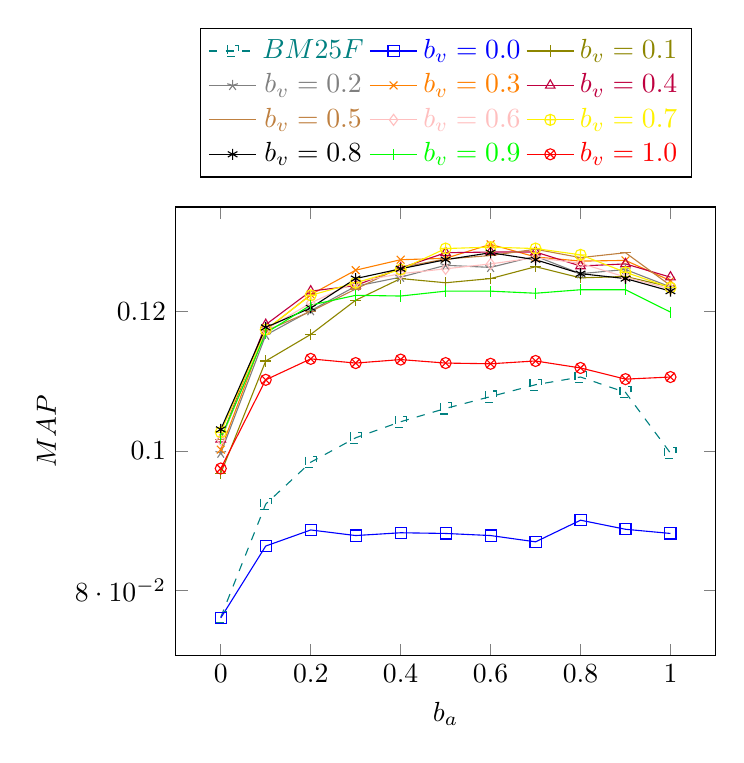
\begin{tikzpicture}
\begin{axis}[
  legend entries={
    [teal]$BM25F$,
	[blue]$b_v = 0.0$,
 	[olive]$b_v = 0.1$,
  	[gray]$b_v = 0.2$,
  	[orange]$b_v = 0.3$,
	[purple]$b_v = 0.4$,
 	[brown]$b_v = 0.5$,
  	[pink]$b_v = 0.6$,
  	[yellow]$b_v = 0.7$,
	[black]$b_v = 0.8$,
 	[green]$b_v = 0.9$,
 	[red]$b_v = 1.0$
  },
  legend columns=3,
legend style={at={(0.5,1.4)},anchor=north},
 xlabel=$b_a$,
ylabel=$MAP$,
% y label style={rotate=-90},
]

%%%%%%%%%%%
%% x = c_v, y = c_a
%%%%%%%%%%%
%\addplot[mark=square, style=solid, color=blue] coordinates
%{ (0.0, 0.0761) (0.1, 0.0968) (0.2, 0.0997) (0.3, 0.1002) (0.4, 0.1017) (0.5, 0.1016) (0.6, 0.1016) (0.7, 0.1027) (0.8, 0.1031) (0.9, 0.1018) (1.0, 0.0975) };

%\addplot[mark=+, style=solid, color=olive] coordinates
%{ (0.0, 0.0864) (0.1, 0.1129) (0.2, 0.1166) (0.3, 0.1173) (0.4, 0.1181) (0.5, 0.1172) (0.6, 0.1174) (0.7, 0.1174) (0.8, 0.1177) (0.9, 0.1169) (1.0, 0.1102) };

%\addplot[mark=star, style=solid, color=gray] coordinates
%{ (0.0, 0.0887) (0.1, 0.1167) (0.2, 0.1201) (0.3, 0.1224) (0.4, 0.1229) (0.5, 0.12) (0.6, 0.1212) (0.7, 0.1223) (0.8, 0.1205) (0.9, 0.1209) (1.0, 0.1132) };

%\addplot[mark=x, style=solid, color=orange] coordinates
%{ (0.0, 0.0879) (0.1, 0.1216) (0.2, 0.1236) (0.3, 0.1259) (0.4, 0.1237) (0.5, 0.1232) (0.6, 0.1242) (0.7, 0.1241) (0.8, 0.1247) (0.9, 0.1223) (1.0, 0.1126) };

%\addplot[mark=triangle, style=solid, color=purple] coordinates
%{ (0.0, 0.0883) (0.1, 0.1247) (0.2, 0.1249) (0.3, 0.1274) (0.4, 0.1262) (0.5, 0.1263) (0.6, 0.1254) (0.7, 0.126) (0.8, 0.1261) (0.9, 0.1222) (1.0, 0.1131) };

%\addplot[mark=-, style=solid, color=brown] coordinates
%{ (0.0, 0.0882) (0.1, 0.1241) (0.2, 0.1266) (0.3, 0.1276) (0.4, 0.1284) (0.5, 0.1275) (0.6, 0.1261) (0.7, 0.129) (0.8, 0.1274) (0.9, 0.1229) (1.0, 0.1126) };

%\addplot[mark=diamond, style=solid, color=pink] coordinates
%{ (0.0, 0.0879) (0.1, 0.1247) (0.2, 0.1263) (0.3, 0.1296) (0.4, 0.1285) (0.5, 0.128) (0.6, 0.1268) (0.7, 0.1292) (0.8, 0.1284) (0.9, 0.1229) (1.0, 0.1125) };

%\addplot[mark=oplus, style=solid, color=yellow] coordinates
%{ (0.0, 0.087) (0.1, 0.1264) (0.2, 0.1279) (0.3, 0.1278) (0.4, 0.1285) (0.5, 0.1289) (0.6, 0.1277) (0.7, 0.129) (0.8, 0.1274) (0.9, 0.1226) (1.0, 0.1129) };

%\addplot[mark=asterisk, style=solid, color=black] coordinates
%{ (0.0, 0.0901) (0.1, 0.1248) (0.2, 0.1254) (0.3, 0.1272) (0.4, 0.1265) (0.5, 0.1277) (0.6, 0.1269) (0.7, 0.1281) (0.8, 0.1254) (0.9, 0.1231) (1.0, 0.1119) };

%\addplot[mark=|, style=solid, color=green] coordinates
%{ (0.0, 0.0888) (0.1, 0.125) (0.2, 0.126) (0.3, 0.1273) (0.4, 0.1268) (0.5, 0.1284) (0.6, 0.1249) (0.7, 0.1256) (0.8, 0.1247) (0.9, 0.1231) (1.0, 0.1103) };

%\addplot[mark=otimes, style=solid, color=red] coordinates
%{ (0.0, 0.0882) (0.1, 0.1235) (0.2, 0.1235) (0.3, 0.1244) (0.4, 0.1249) (0.5, 0.1237) (0.6, 0.1232) (0.7, 0.1234) (0.8, 0.1229) (0.9, 0.1199) (1.0, 0.1106) };

%%%%%%%%%%%
%% x = b_a, y = b_v
%%%%%%%%%%%
\addplot[mark=square, style=dashed, color=teal] coordinates
{ (0, 0.0762) (.1, 0.0924) (.2, 0.0984) (.3, 0.1019) (.4, 0.1042) (.5, 0.1061) (.6, 0.1078) (.7, 0.1095) (.8, 0.1106) (.9, 0.1084) (1.0, 0.0997) };

\addplot[mark=square, style=solid, color=blue] coordinates
{ (0.0, 0.0761) (0.1, 0.0864) (0.2, 0.0887) (0.3, 0.0879) (0.4, 0.0883) (0.5, 0.0882) (0.6, 0.0879) (0.7, 0.087) (0.8, 0.0901) (0.9, 0.0888) (1.0, 0.0882) };

\addplot[mark=+, style=solid, color=olive] coordinates
{ (0.0, 0.0968) (0.1, 0.1129) (0.2, 0.1167) (0.3, 0.1216) (0.4, 0.1247) (0.5, 0.1241) (0.6, 0.1247) (0.7, 0.1264) (0.8, 0.1248) (0.9, 0.125) (1.0, 0.1235) };

\addplot[mark=star, style=solid, color=gray] coordinates
{ (0.0, 0.0997) (0.1, 0.1166) (0.2, 0.1201) (0.3, 0.1236) (0.4, 0.1249) (0.5, 0.1266) (0.6, 0.1263) (0.7, 0.1279) (0.8, 0.1254) (0.9, 0.126) (1.0, 0.1235) };

\addplot[mark=x, style=solid, color=orange] coordinates
{ (0.0, 0.1002) (0.1, 0.1173) (0.2, 0.1224) (0.3, 0.1259) (0.4, 0.1274) (0.5, 0.1276) (0.6, 0.1296) (0.7, 0.1278) (0.8, 0.1272) (0.9, 0.1273) (1.0, 0.1244) };

\addplot[mark=triangle, style=solid, color=purple] coordinates
{ (0.0, 0.1017) (0.1, 0.1181) (0.2, 0.1229) (0.3, 0.1237) (0.4, 0.1262) (0.5, 0.1284) (0.6, 0.1285) (0.7, 0.1285) (0.8, 0.1265) (0.9, 0.1268) (1.0, 0.1249) };

\addplot[mark=-, style=solid, color=brown] coordinates
{ (0.0, 0.1016) (0.1, 0.1172) (0.2, 0.12) (0.3, 0.1232) (0.4, 0.1263) (0.5, 0.1275) (0.6, 0.128) (0.7, 0.1289) (0.8, 0.1277) (0.9, 0.1284) (1.0, 0.1237) };

\addplot[mark=diamond, style=solid, color=pink] coordinates
{ (0.0, 0.1016) (0.1, 0.1174) (0.2, 0.1212) (0.3, 0.1242) (0.4, 0.1254) (0.5, 0.1261) (0.6, 0.1268) (0.7, 0.1277) (0.8, 0.1269) (0.9, 0.1249) (1.0, 0.1232) };

\addplot[mark=oplus, style=solid, color=yellow] coordinates
{ (0.0, 0.1027) (0.1, 0.1174) (0.2, 0.1223) (0.3, 0.1241) (0.4, 0.126) (0.5, 0.129) (0.6, 0.1292) (0.7, 0.129) (0.8, 0.1281) (0.9, 0.1256) (1.0, 0.1234) };

\addplot[mark=asterisk, style=solid, color=black] coordinates
{ (0.0, 0.1031) (0.1, 0.1177) (0.2, 0.1205) (0.3, 0.1247) (0.4, 0.1261) (0.5, 0.1274) (0.6, 0.1284) (0.7, 0.1274) (0.8, 0.1254) (0.9, 0.1247) (1.0, 0.1229) };

\addplot[mark=|, style=solid, color=green] coordinates
{ (0.0, 0.1018) (0.1, 0.1169) (0.2, 0.1209) (0.3, 0.1223) (0.4, 0.1222) (0.5, 0.1229) (0.6, 0.1229) (0.7, 0.1226) (0.8, 0.1231) (0.9, 0.1231) (1.0, 0.1199) };

\addplot[mark=otimes, style=solid, color=red] coordinates
{ (0.0, 0.0975) (0.1, 0.1102) (0.2, 0.1132) (0.3, 0.1126) (0.4, 0.1131) (0.5, 0.1126) (0.6, 0.1125) (0.7, 0.1129) (0.8, 0.1119) (0.9, 0.1103) (1.0, 0.1106) };

\end{axis}
\end{tikzpicture}}

	\caption{SS10}
\end{subfigure}
\quad%
\begin{subfigure}[b]{.3\textwidth}
\centering
\resizebox{\textwidth}{!}{
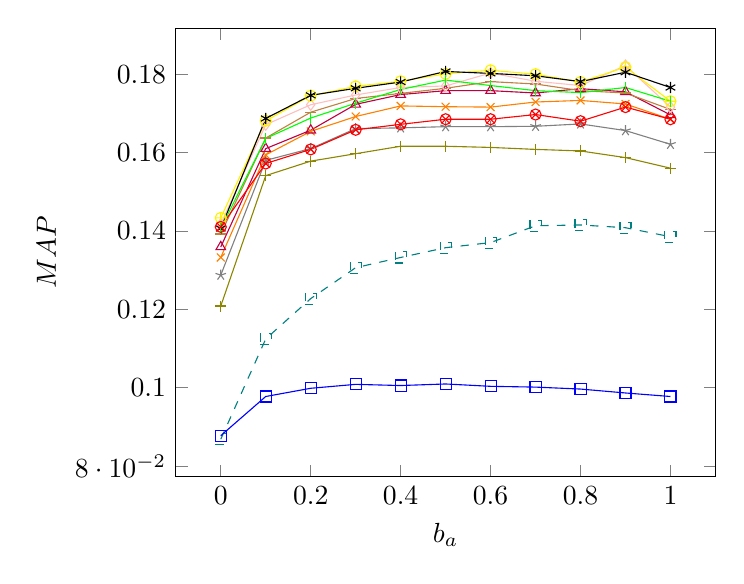
\begin{tikzpicture}
\begin{axis}[
 xlabel=$b_a$,
ylabel=$MAP$,
% y label style={rotate=-90},
]

%%%%%%%%%%%
%% x = b_v, y = b_a
%%%%%%%%%%%
%\addplot[mark=square, style=solid, color=blue] coordinates
%{ (0.0,  0.0877) (0.1,  0.1208) (0.2,  0.1287) (0.3,  0.1332) (0.4,  0.1359) (0.5,  0.1392) (0.6,  0.1417) (0.7,  0.1433) (0.8, 0.1406) (0.9, 0.1406) (1.0, 0.141) };

%\addplot[mark=+, style=solid, color=olive] coordinates
%{ (0.0,  0.0977) (0.1, 0.1541 ) (0.2,  0.158) (0.3, 0.1594) (0.4,  0.161) (0.5,  0.1637) (0.6, 0.1671) (0.7,  0.1681) (0.8, 0.1687) (0.9,  0.1636) (1.0,  0.1572) };

%\addplot[mark=star, style=solid, color=gray] coordinates
%{ (0.0, 0.0998 ) (0.1,  0.1578) (0.2,  0.161) (0.3,  0.1654) (0.4,  0.1657) (0.5, 0.1703) (0.6,  0.1722) (0.7, 0.1745) (0.8,  0.1746) (0.9,  0.1688) (1.0, 0.1608) };

%\addplot[mark=x, style=solid, color=orange] coordinates
%{ (0.0,  0.1008) (0.1,  0.1597) (0.2,  0.1661) (0.3,  0.1692) (0.4,  0.1723) (0.5, 0.1738) (0.6, 0.1747) (0.7, 0.1769) (0.8,  0.1764) (0.9,  0.1726) (1.0, 0.1658) };

%\addplot[mark=triangle, style=solid, color=purple] coordinates
%{ (0.0,  0.1005) (0.1,  0.1616) (0.2,  0.1663) (0.3,  0.1719) (0.4, 0.1748 ) (0.5, 0.1751) (0.6,0.1766 ) (0.7, 0.1782) (0.8,  0.178) (0.9,  0.1761) (1.0,  0.1672) };

%\addplot[mark=-, style=solid, color=brown] coordinates
%{ (0.0,  0.1009) (0.1,  0.1616) (0.2,  0.1666) (0.3,  0.1717) (0.4,  0.1758) (0.5, 0.1764 ) (0.6, 0.177) (0.7, 0.1801) (0.8,  0.1807) (0.9,  0.1785) (1.0, 0.1685) };

%\addplot[mark=diamond, style=solid, color=pink] coordinates
%{ (0.0,  0.1003) (0.1,  0.1613) (0.2,  0.1666) (0.3,  0.1716) (0.4,  0.1758) (0.5, 0.1781) (0.6, 0.1803) (0.7, 0.181) (0.8,  0.1802) (0.9,  0.1771) (1.0,  0.1685) };

%\addplot[mark=oplus, style=solid, color=yellow] coordinates
%{ (0.0,  0.1001) (0.1,  0.1608) (0.2,  0.1667) (0.3,  0.1729) (0.4,  0.1752) (0.5, 0.1775) (0.6, 0.1782) (0.7, 0.18) (0.8, 0.1796 ) (0.9,  0.1758) (1.0,  0.1697) };

%\addplot[mark=asterisk, style=solid, color=black] coordinates
%{ (0.0, 0.0996 ) (0.1,  0.1604) (0.2, 0.1673 ) (0.3, 0.1733 ) (0.4, 0.1763 ) (0.5, 0.1758 ) (0.6, 0.1771) (0.7, 0.178) (0.8,  0.1781) (0.9,  0.1753) (1.0,  0.168) };

%\addplot[mark=|, style=solid, color=green] coordinates
%{ (0.0,  0.0986) (0.1, 0.1587 ) (0.2, 0.1656 ) (0.3, 0.1724 ) (0.4, 0.1755 ) (0.5, 0.1752 ) (0.6, 0.1822) (0.7, 0.1818) (0.8, 0.1805 ) (0.9, 0.1766 ) (1.0, 0.1716 )
%};

%\addplot[mark=otimes, style=solid, color=red] coordinates
%{ (0.0, 0.0977 ) (0.1, 0.156 ) (0.2, 0.1621 ) (0.3, 0.1685 ) (0.4, 0.1696 ) (0.5, 0.171 ) (0.6, 0.1716 ) (0.7, 0.1731 ) (0.8, 0.1766) (0.9, 0.1731) (1.0, 0.1685 ) };

%%%%%%%%%%%
%% x = b_a, y = b_v
%%%%%%%%%%%

\addplot[mark=square, style=dashed, color=teal] coordinates
{ (0, 0.0868) (.1, 0.1124) (.2, 0.1227) (.3, 0.1306) (.4, 0.1332) (.5, 0.1357) (.6, 0.137) (.7, 0.1413) (.8, 0.1415) (.9, 0.1408) (1.0, 0.1385) };

\addplot[mark=square, style=solid, color=blue] coordinates
{ (0.0, 0.0877) (0.1, 0.0977) (0.2, 0.0998) (0.3, 0.1008) (0.4, 0.1005) (0.5, 0.1009) (0.6, 0.1003) (0.7, 0.1001) (0.8, 0.0996) (0.9, 0.0986) (1.0, 0.0977) };

\addplot[mark=+, style=solid, color=olive] coordinates
{ (0.0, 0.1208) (0.1, 0.1541) (0.2, 0.1578) (0.3, 0.1597) (0.4, 0.1616) (0.5, 0.1616) (0.6, 0.1613) (0.7, 0.1608) (0.8, 0.1604) (0.9, 0.1587) (1.0, 0.156) };

\addplot[mark=star, style=solid, color=gray] coordinates
{ (0.0, 0.1287) (0.1, 0.158) (0.2, 0.161) (0.3, 0.1661) (0.4, 0.1663) (0.5, 0.1666) (0.6, 0.1666) (0.7, 0.1667) (0.8, 0.1673) (0.9, 0.1656) (1.0, 0.1621) };

\addplot[mark=x, style=solid, color=orange] coordinates
{ (0.0, 0.1332) (0.1, 0.1594) (0.2, 0.1654) (0.3, 0.1692) (0.4, 0.1719) (0.5, 0.1717) (0.6, 0.1716) (0.7, 0.1729) (0.8, 0.1733) (0.9, 0.1724) (1.0, 0.1685) };

\addplot[mark=triangle, style=solid, color=purple] coordinates
{ (0.0, 0.1359) (0.1, 0.161) (0.2, 0.1657) (0.3, 0.1723) (0.4, 0.1748) (0.5, 0.1758) (0.6, 0.1758) (0.7, 0.1752) (0.8, 0.1763) (0.9, 0.1755) (1.0, 0.1696) };

\addplot[mark=-, style=solid, color=brown] coordinates
{ (0.0, 0.1392) (0.1, 0.1637) (0.2, 0.1703) (0.3, 0.1738) (0.4, 0.1751) (0.5, 0.1764) (0.6, 0.1781) (0.7, 0.1775) (0.8, 0.1758) (0.9, 0.1752) (1.0, 0.171) };

\addplot[mark=diamond, style=solid, color=pink] coordinates
{ (0.0, 0.1417) (0.1, 0.1671) (0.2, 0.1722) (0.3, 0.1747) (0.4, 0.1766) (0.5, 0.177) (0.6, 0.1803) (0.7, 0.1782) (0.8, 0.1771) (0.9, 0.1822) (1.0, 0.1716) };

\addplot[mark=oplus, style=solid, color=yellow] coordinates
{ (0.0, 0.1433) (0.1, 0.1681) (0.2, 0.1745) (0.3, 0.1769) (0.4, 0.1782) (0.5, 0.1801) (0.6, 0.181) (0.7, 0.18) (0.8, 0.178) (0.9, 0.1818) (1.0, 0.1731) };

\addplot[mark=asterisk, style=solid, color=black] coordinates
{ (0.0, 0.1406) (0.1, 0.1687) (0.2, 0.1746) (0.3, 0.1764) (0.4, 0.178) (0.5, 0.1807) (0.6, 0.1802) (0.7, 0.1796) (0.8, 0.1781) (0.9, 0.1805) (1.0, 0.1766) };

\addplot[mark=|, style=solid, color=green] coordinates
{ (0.0, 0.1406) (0.1, 0.1636) (0.2, 0.1688) (0.3, 0.1726) (0.4, 0.1761) (0.5, 0.1785) (0.6, 0.1771) (0.7, 0.1758) (0.8, 0.1753) (0.9, 0.1766) (1.0, 0.1731) };

\addplot[mark=otimes, style=solid, color=red] coordinates
{ (0.0, 0.141) (0.1, 0.1572) (0.2, 0.1608) (0.3, 0.1658) (0.4, 0.1672) (0.5, 0.1685) (0.6, 0.1685) (0.7, 0.1697) (0.8, 0.168) (0.9, 0.1716) (1.0, 0.1685) };

\end{axis}
\end{tikzpicture}}
\caption{SS11}
\end{subfigure}
\caption{Experiment with the BM25MF normalization parameters. The figures report the MAP values of the respective datasets, where a curve plots a fixed $b_v$ value with $b_a$ varying from $0$ to $1$ with a precision step of $0.1$.}
\label{fig:bm25mf-norm}
\end{figure}
